%\vspace{1.5pc}
\vspace{1.5pc}
%\section[State of the Art]{State of the Art}
\begin{spacing}{1.5}
	
	Bab ini menjelaskan lebih detail mengenai pustaka relevan dan tinjauan teori dalam penelitian ini. Hal ini bertujuan untuk mereview, mengupdate, mengkritik dan mensintesis literatur, melakukan meta-analisis literatur, melakukan konsepsi ulang dari topik yang direview, dan menjawab pertanyaan spesifik penelitian dari topik yang telah direview dalam literatur \shortcite{Torraco2016}. Struktur pembahasan studi relevan dan tinjauan teori selanjutnya dibagi dalam beberapa hal: pertama, akan dibahas mengenai persamaan gerak fluida dan Navier-Stokes dalam pemodelan laut secara umum.
	
	
\end{spacing}
\vspace{-0.1pc}
\section[Persamaan Gerak Fluida]{Persamaan Gerak Fluida}
\begin{spacing}{1.5}
	
	Persamaan matematika yang mengatur aliran viskoelastik fluida berasal dari persamaan-persamaan hukum konservasi fisika yaitu konservasi massa, momentum dan persamaan konstitutif reologi \shortcite{Alves2021}. Penjabaran dari hukum-hukum tersebut menentukan bagaimana suatu persamaan model hidrodinamika dibuat. Salah satu persamaan fluida yang paling terkenal adalah persamaan Navier-Stokes yang terdiri dari persamaan momentum, persamaan kontinuitas, dan persamaan kekekalan densitas \shortcite{Haditiar2020}. Persamaan Navier-Stokes digunakan untuk menggambarkan fluida yang mengalir dan dianggap memiliki pergerakan yang kontinu. Diketahui bahwa hasil pengamatan dari sebuah partikel fluida yang mengalir memiliki sifat-sifat fluida secara umum yaitu kecepatan, temperatur, tekanan dan densitas \shortcite{Rafiq2019,Das2018,Khan2019}. Sebuah partikel fluida diilustrasikan pada Gambar \ref{fig:cube}a, dan \ref{fig:cube}b. Komponen fluida seperti tekanan $p$, kecepatan $u$, dan densitas $\rho$ terletak pada pusat partikel yang bergantung terhadap waktu $(t)$ dan ruang $(x,y,z)$. Sehingga, komponen-komponen tersebut dapat ditulis dalam fungsi $p(x,y,z,t), u(x,y,z,t)$  dan $\rho(x,y,z,t)$. 
	
	\begin{figure}[H]
		\centering
		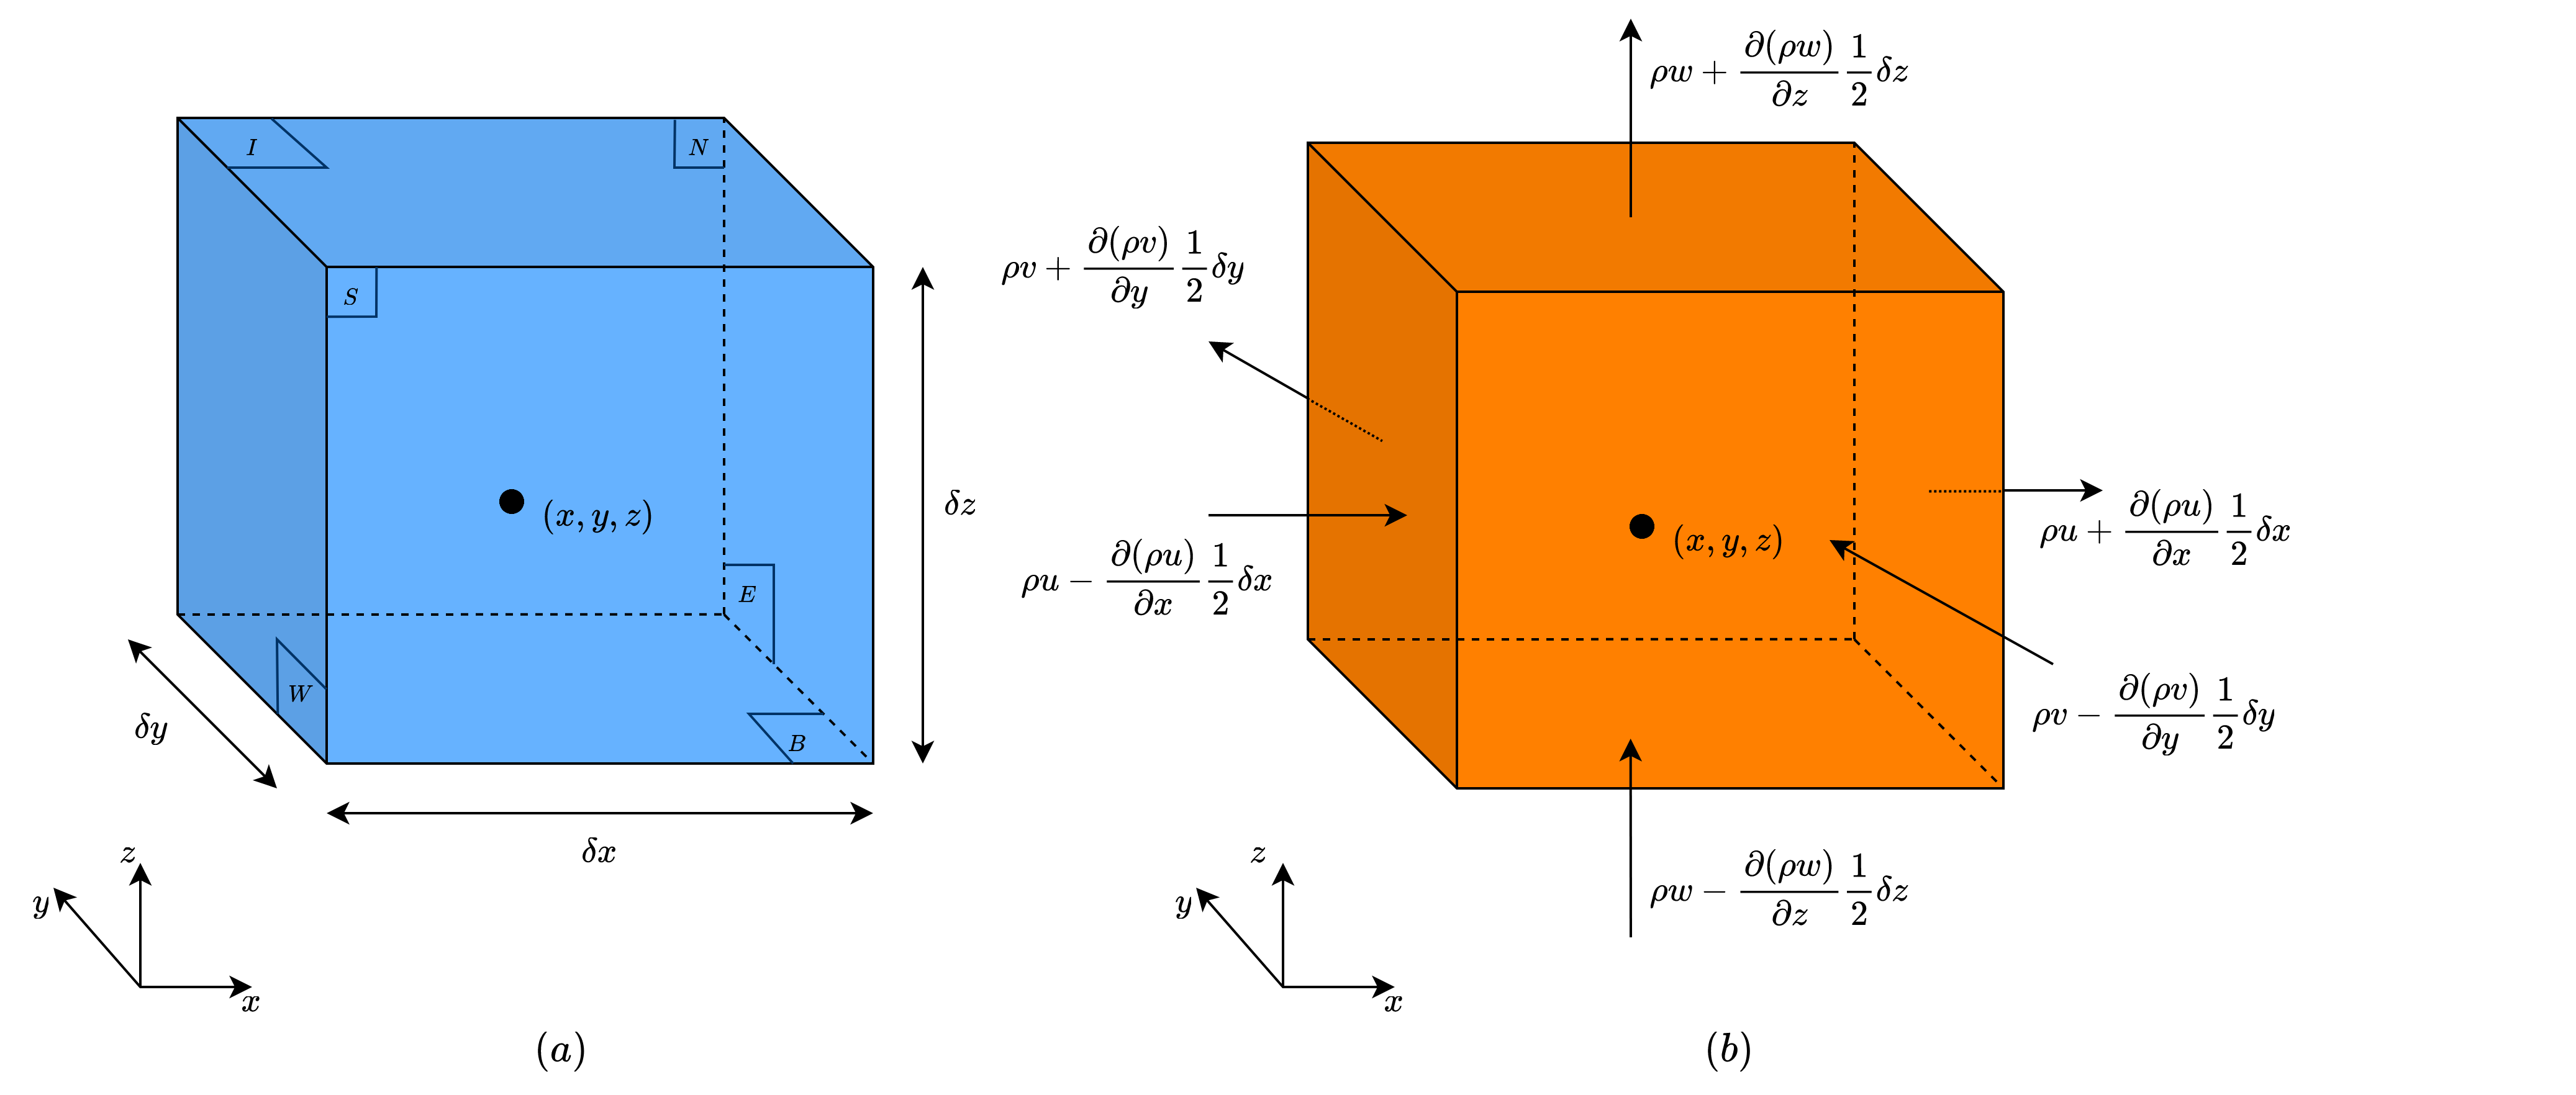
\includegraphics[width=16cm]{contents/cube}
		\caption{(a) Ilustrasi partikel sebagai sifat fisis fluida. (b) Aliran massa jenis masuk dan keluar \protect\shortcite{versteeg2007introduction}}
		\label{fig:cube}
		\medspace
		\small
		Massa jenis dari partikel $\rho(x,y,z,t)$ pada gambar bagian (a) dapat diterjemahkan sebagai aliran yang masuk dan keluar. Pada gambar bagian (b), arah aliran massa jenis pada partikel pusat merupakan jumlahan dari aliran massa jenis masuk dan keluar. Dengan cara yang sama, dapat juga dilakukan untuk tekanan dan kecepatan. 
	\end{figure}
	
\end{spacing}
\vspace{-1pc}
\section[Persamaan Navier-Stokes 3 Dimensi]{Persamaan Navier-Stokes 3 Dimensi}
\begin{spacing}{1.5}
	\par Model sirkulasi laut atau \textit{Ocean General Circulation Models} (OGCM) menggunakan persamaan Navier-Stokes untuk memodelkan fenomena fisis yang terjadi di lautan. Persamaan gerak Navier-Stokes nonhidrostatik dalam model 3-D terdiri dari persamaan momentum, persamaan kontinuitas, dan persamaan konservasi densitas \shortcite{Haditiar2020}. Pada model Navier-Stokes dengan pendekatan nonhidrostatik, tekanan air laut (P) dipecah menjadi dua bagian utama, yaitu: tekanan hidrostatik (p) dan tekanan nonhidrostatik (q)
	\begin{equation}
		P = p+q.
	\end{equation}
	Tekanan p dihitung secara diagnostik dari densitas  dan percepatan gravitasi g seperti pada persamaan berikut 
	\begin{equation}
		\frac{\partial p}{\partial z} = -(\rho - \rho_0)g.
	\end{equation}
	Sedangkan tekanan q dihitung secara prognostik dalam persamaan momentum (implisit). Hal ini karena tekanan q bergantung terhadap sirkulasi arus.
	\par Persamaan momentum lengkap untuk model nonhidrostatik adalah sebagai berikut
	\begin{equation}
		\begin{aligned}
			\frac{\partial u}{\partial t} + \text{adv}(u)-fv &= \frac{-1}{\rho_0}\frac{\partial(p+q)}{\partial x}+\text{diff}(u) \\
			\frac{\partial v}{\partial t} + \text{adv}(v)+fu &= \frac{-1}{\rho_0}\frac{\partial(p+q)}{\partial y}+\text{diff}(v) \\
			\frac{\partial w}{\partial t} +\text{adv}(w) &= \frac{-1}{\rho_0}\frac{\partial(q)}{\partial y}+\text{diff}(w).
		\end{aligned}	
	\end{equation}
	\par Dengan $\text{adv}(\psi)=u\frac{\partial \psi}{\partial x}+v\frac{\partial \psi}{\partial y}+w\frac{\partial \psi}{\partial z}$ adalah persamaan adveksi dan $\text{diff}(\psi)=\frac{\partial}{\partial x}(A_{H} \frac{\partial \psi}{\partial x})+\frac{\partial}{\partial y}(A_{H} \frac{\partial \psi}{\partial y})+\frac{\partial}{\partial z}(A_{Z} \frac{\partial \psi}{\partial z})$ adalah persamaan difusi dengan $A_H$ dan $A_Z$ koefisien gesekan eddy horizontal dan vertikal. 
	\par Kecepatan arus dalam sistem koordinat Cartesian 3-D didefinisikan dengan u,v, dan w. Waktu didefinisikan dengan t, parameter Coriolis dengan f, dan densitas air laut referensi dengan $\rho_0$.
	Untuk persamaan kontinuitas atau kekekalan volume diekspresikan dalam persamaan berikut
	\begin{equation}
		\frac{\partial u}{\partial t} + \frac{\partial v}{\partial t} + \frac{\partial w}{\partial t} = 0.
	\end{equation}
	Berdasarkan persamaan kontinuitas (2.4), tekanan dinamis pada lapisan permukaan dapat dihitung dengan persamaan berikut
	\begin{equation}
		\frac{\partial q_s}{\partial t} = \rho_0 g_i \times \left( \frac{(\partial \left(H \langle u \rangle \right)} {\partial x} + \frac{(\partial \left(H \langle v \rangle \right)} {\partial y}\right)
	\end{equation}
	dengan $q_s = \rho_0 g \eta$. Disini $\rho_0$ adalah densitas air laut referensi, dan $\eta$ adalah elevasi permukaan laut, $H$ adalah total kedalaman laut, dan $< >$ adalah operator rata-rata vertikal.
	\par Densitas air laut bergantung pada temperatur, salinitas, dan tekanan. Selanjutnya asumsikan bahwa air laut hanya bergantung linear terhadap temperatur dan salinitas, serta difusifitas \textit{eddy} untuk temperatur dan salinitas sama. Persamaan konservasi densitas diberikan oleh,
	\begin{equation}
		\frac{\partial \rho}{\partial t} + \text{adv}(\rho) = \text{diff}(\rho).
	\end{equation}
	Dalam aplikasinya, persamaan Navier-Stokes tidak hanya digunakan untuk memodelkan laut, tapi juga merambah ke bidang pemodelan cuaca \shortcite{Rohli2021}, aliran air dalam pipa \shortcite{Ouchiha2012} dan aliran udara di sekitar sayap pesawat \shortcite{Tulus2019}. Dalam bentuk persamaan lengkap dan simplifikasi, persamaan ini juga dapat digunakan untuk mendesain kereta api \shortcite{Croquer2020}, pesawat terbang \shortcite{Chau2021}, dan mobil \shortcite{Ambarita2018}. Terdapat juga studi tentang aliran darah \shortcite{Gill2021}, desain stasiun pembangkit listrik \shortcite{Yang2019}, dan analisis polusi udara \shortcite{Issakhov2022}. 
\end{spacing}
\vspace{-0.1pc}
\section[Model Iklim]{Model Iklim}
\begin{spacing}{1.5}
\end{spacing}
	
